%
% $Id: ch04_implementation.tex
%
%   *******************************************************************
%   * SEE THE MAIN FILE "AllegThesis.tex" FOR MORE INFORMATION.       *
%   *******************************************************************
%
\chapter{Experimental Results}\label{ch:results}

In this chapter, we will discuss our method of verifying the accuracy of our system,
a discussion of our case study, an analysis of the results produced by our system,
and a listing of possible threats to the validity of our results.

\section{Testing}\label{sec:test}

Throughout the development process, we used several mechanisms to verify the accuracy
of our system.  Prior to starting implementation, we selected a very simple sample
program to ensure that we could use CodeCover to produce per-test coverage data.  The
program we selected was a small system developed by Nathaniel Blake, Tristan Challener, 
and Eric Weyant as a course project at Allegheny College.  The system consists of four
source files and eleven JUnit test cases, and has functionality related to file input,
list manipulation, and CSV output.  We selected this application primarily for its
simplicity, existing JUnit test suite, and our familiarity with the code.  Its
simplicity allowed us to easily import the system to Eclipse and set up the environment
to successfully run all included tests.  This process was aided by our familiarity with
the code and tests; although we did not have to modify any executable code or the 
content of any tests, we were required to update certain aspects of the tests to behave
correctly on a Windows operating system.

After importing our selected application into Eclipse, we installed the most recent version
of the CodeCover Eclipse plugin.  By following directions provided in the CodeCover documentation,
we were able to execute the application through CodeCover and produce per-test coverage data.
Because CodeCover containers are internal mechanisms for storing coverage data and are not
meant to be viewed directly, there is very little documentation available.  As such, we were 
forced to examine the container output to determine its structure before developing parsing
tools.  See Section \ref{sec:ir} for additional details about the content of CodeCover
container files.

As we proceeded with the implementation described in Chapter \ref{ch:method}, we cross-checked
the data produced from our parse tool with that available through interacting with the CodeCover
Eclipse plugin.  We were able to verify that our parsed coverage data was consistent
with the data shown in Eclipse.  Verifiable data included statement source code, execution 
counts for each statement, and test case pass/fail status.  In addition, we verified the values
generated for $ae_p, ae_f, an_p,$ and $an_f$ through manually totaling the number of appearances 
of each statement in the container coverage segment to the values of each of the aforementioned
variables.  

Through these processes we were able to establish a reasonable level of confidence
in the correctness of our system.  Automated testing was not a feasible option for this process
due to the complex nature of the container being parsed, since any testing would require 
repeating the parsing process---thereby negating the benefits of the test.  Automated testing
was used, however, to verify the accuracy of the risk evaluation function implementations
used in the system.  We designed table-driven JUnit tests with multiple test inputs to 
ensure that all functions were correctly implemented within a reasonable degree of confidence.

\section{Case Study}\label{sec:case}

In order to provide further evidence for the accuracy of our system and to produce preliminary 
comparison data for our tested risk evaluation functions, we performed a case study with another
selected application. Due to the simplicity of the test application described in Section \ref{sec:test}, 
we chose a different case application for our study.  The program we selected is Jni-InChi
\cite{jniinchi}, which ``enables Java software to generate IUPAC's International Chemical Identifiers 
(InChIs) by making Java Native Interface (JNI) calls to the InChI C library developed by IUPAC''.

This application, along with several others, was prepared and executed through MAJOR by Sarojini
Balasubramanian.  The mutation data were provided as well.  We selected this application, from the
several other applications available, due to limitations of CodeCover that were not clear until we
began testing various applications.  Many tested applications had passing JUnit test suites after
being imported to Eclipse, but still produced the following (or similar) error when we attempted
to run them through CodeCover:

\vspace{5mm}
\texttt{[FATAL] An error occurred when trying to compile the instrumented sources.}
\vspace{2mm}

According to a discussion post at the CodeCover \texttt{sourceforge}
page, made by CodeCover developer Tilmann Scheller \cite{discpost}, there is not currently any 
means of producing more verbose output (including details on compiler errors) through Eclipse.  
Additional discussion indicated that CodeCover is able to ``instrument
a single source directory only.''  Since the majority of the projects provided and executed with MAJOR
feature several source directories, we were severely limited in choice of case study application.  
Fortunately, the Jni-InChi project includes only a single source directory and we were able
to generate CodeCover output for this system.

\begin{figure}
\centering
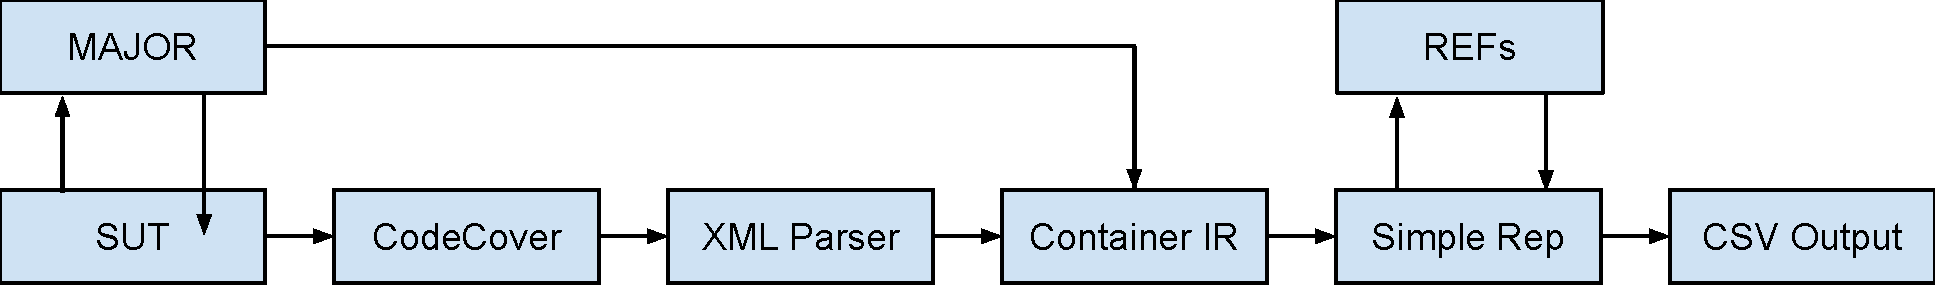
\includegraphics[width=0.9\linewidth]{img/Architecture.pdf}
\caption{The overall architecture of the system for experimentation.  The system under test (SUT) is executed through MAJOR, and some fault is inserted.  The SUT then passed through CodeCover, and the resulting container forms the input to the XML parser.  The parsed container, and the fault, are passed into the IR builder.  Once the IR is built, it is passed to the simplified representation (SR) modifier.  The SR calls all of the necessary risk evaluation functions (REFs), then outputs the results to CSV.}
\label{fig:arch}
\end{figure}

In order to produce meaningful results, the CodeCover execution of JUnit must complete or no coverage
data is written the container.  Additionally, the JUnit test must
feature at least one failure---otherwise no
suspiciousness information can be generated.  To achieve this, we repeatedly selected
arbitrary \textit{killed} mutants generated by MAJOR (their killed status guarantees at least one failed
test case).  As mentioned earlier, mutants have been shown to be representative of real-world faults.  
Specifically, mutants generated using MAJOR were shown to be representative in the study by Just et al.
\cite{mutants}  The overall layout of this test is visualized in Figure \ref{fig:arch}.

\begin{figure}[tb]
\begin{lstlisting}
119:ROR:==(java.lang.Object,java.lang.Object):
	FALSE(java.lang.Object,java.lang.Object):
	net.sf.jniinchi.JniInchiAtom@<init>:117:el == null |==> false
137:STD:<CALL>:<NO-OP>:
	net.sf.jniinchi.JniInchiStructure@addBond:99:
	bondList.add(bond) |==> <NO-OP>
149:LVR:POS:NEG:
	net.sf.jniinchi.JniInchiStereo0D@<init>:79:3 |==> -3
194:COR:||(boolean,boolean):LHS(boolean,boolean):
	net.sf.jniinchi.JniInchiWrapper@checkOptions:183:
	op.startsWith("-") || op.startsWith("/") |==> op.startsWith("-")
197:STD:<CALL>:<NO-OP>:
	net.sf.jniinchi.JniInchiWrapper@checkOptions:189:
	sbOptions.append(flagChar + option.name()) |==> <NO-OP>
\end{lstlisting}

\caption{Mutants selected for use in case study.}
\label{fig:mutants}
\end{figure}

There were various complications that forced us to reject mutants.  First, any mutant that
causes the Eclipse JUnit \texttt{TestRunner} to crash prematurely and not complete the entire test 
suite could not be used.  This is due to meaningless or incomplete coverage data, which is not useful
for generating suspiciousness data.  In many cases, if the \texttt{TestRunner} crashed prematurely,
CodeCover would not write \emph{any} coverage data to the test session container.  Thus, we skipped
any mutants with this property. We also passed over any mutants that modify non-executed code, such
as static variable declarations.  
This makes mutants of this type invalid for the purpose of suspiciousness analysis.  Any remaining
mutants were considered valid.  From those not disqualified, we chose five arbitrary mutants to 
form the basis for this case study.   These mutants can be seen in Figure \ref{fig:mutants}.

Since we only consider basic statements when parsing the CodeCover container, inserted mutants
must be formatted in such a way that they occur as a Java statement and get parsed by CodeCover
as basic statements.  For \texttt{<NO-OP>} mutants such mutant 137, we achieved this by replacing
the listed line with a statement that does nothing.  Specifically, we insert a local variable 
initialization an always-false \texttt{if} statement making use of that variable (if the variable
is never referenced, CodeCover will not recognize the initialization as a basic statement).  That 
variable initialization is treated as the faulty treatment, effectively simulating a no-operation
statement.  Mutants which modify the condition inside an \texttt{if} statement can be represented by 
moving the condition to a boolean variable declared and initialized directly before the \texttt{if}
statement.  That boolean variable initialization is treated as the faulty statement.  The remaining
mutant, number 149 as labeled in Figure \ref{fig:mutants}, requires no additional modifications since
it directly alters a basic statement.

When CodeCover processes source code and builds a test session container, it copies the entire source
code into the container, but removes all comments from the content.  As such, line numbers and character
offsets within CodeCover are not comparable to those within the original source code.  In
order to locate the inserted fault within the container, we require the source code for the faulty
statement to be included as an input to our system, as described in \ref{sec:over}.

\section{Results Analysis}\label{sec:data}

In order to process the data produced by our system for the case application, we made use of the
R functional language for statistical computing \cite{r}.  Since our data already conforms
to tidy data standards \cite{tidy}, and is formatted as CSV, it was relatively simple to import the
data directly into R.  We begin our analysis by reading each CSV results file into a single 
\texttt{data.frame}.  We then vertically merge all of the resulting tables into a single table with
the same variables, but including all observations rather than only those for a single case 
application (mutation).  After merging the tables, we add the EXAM score for each statement to the table 
as a new variable, calculated according to \[EXAM = \frac{Rank}{StatementCount} \times 100.\]

Before making any further use of the data, we create a new table consisting only of the statements
which correspond to the fault.  This is accomplished by selecting only observations from the table
in which the \texttt{IsFault} attribute is true.  We then break this table down into five smaller tables according to the risk evaluation function.  For each of the resulting tables, we extract the 
\texttt{Exam} attribute vector and calculate its mean (the average EXAM value for a given function
across all case applications).  Using these average values, we construct a new table consisting only
of the attributes \texttt{Function} and \texttt{Exam}, made up of five observations---one for each
function and its corresponding average EXAM value.  The final step before visualization is to 
recreate the original five tables, with EXAM values added, by splitting the large table according to
case application.

\begin{figure}[tb]
\centering
\begin{lstlisting}
library( ggplot2 )
attach( jniinchi_119_fault )
graph_119 <- qplot( Function, Exam, data=jniinchi_119_fault, geom="bar", 
			  	ylab="EXAM Score (%)", xlab="Risk Evaulation Function", 
				stat="identity", ylim=c( 0,5 ),
				main="EXAM Score Per Risk Evaluation Function (JniInChi Mutant 119)",
				sub="JniInChi Mutant 119" )
graph_119 <- graph_119 + theme( axis.title=element_text( face="bold.italic" ) )
detach( jniinchi_119_fault )
\end{lstlisting}

\caption{Example code for generating visualization of results.}
\label{fig:rgraph}
\end{figure}

For each of the five case application tables, as well as the average EXAM value table, we produce a
single bar graph.  To do so, we utilize the \texttt{qplot} function from the \texttt{ggplot2} library
\cite{ggplot2}.  The bar graphs plot EXAM score against risk evaluation function, each displaying the
performance of every risk evaluation function for a different case application.  The final graph plots
the average performance of each function across all mutations.  The code used to generate one of the
graphs can be seen in Figure \ref{fig:rgraph}.

\begin{figure}[tb]
\centering
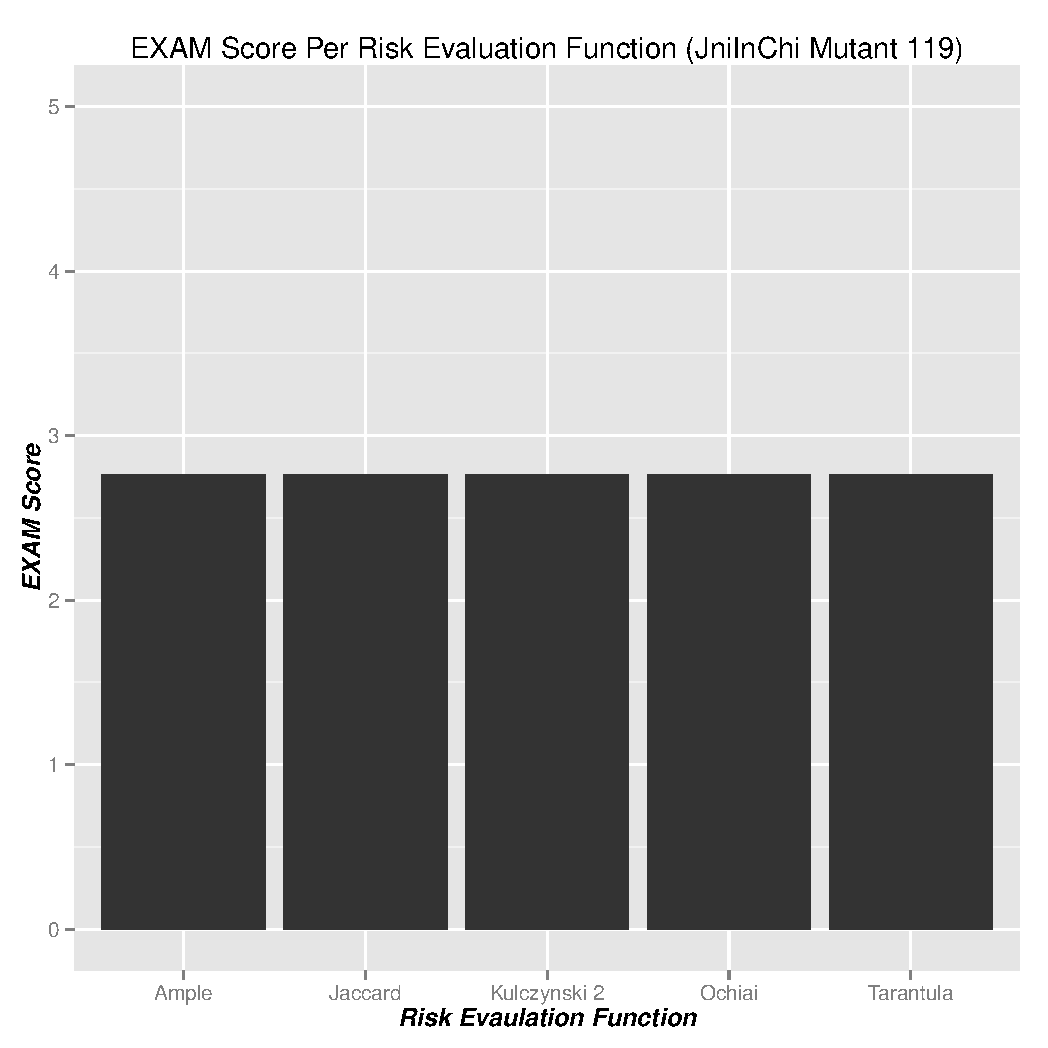
\includegraphics[width=0.4\linewidth]{img/graph_119.pdf}
\hspace{0.1\linewidth}
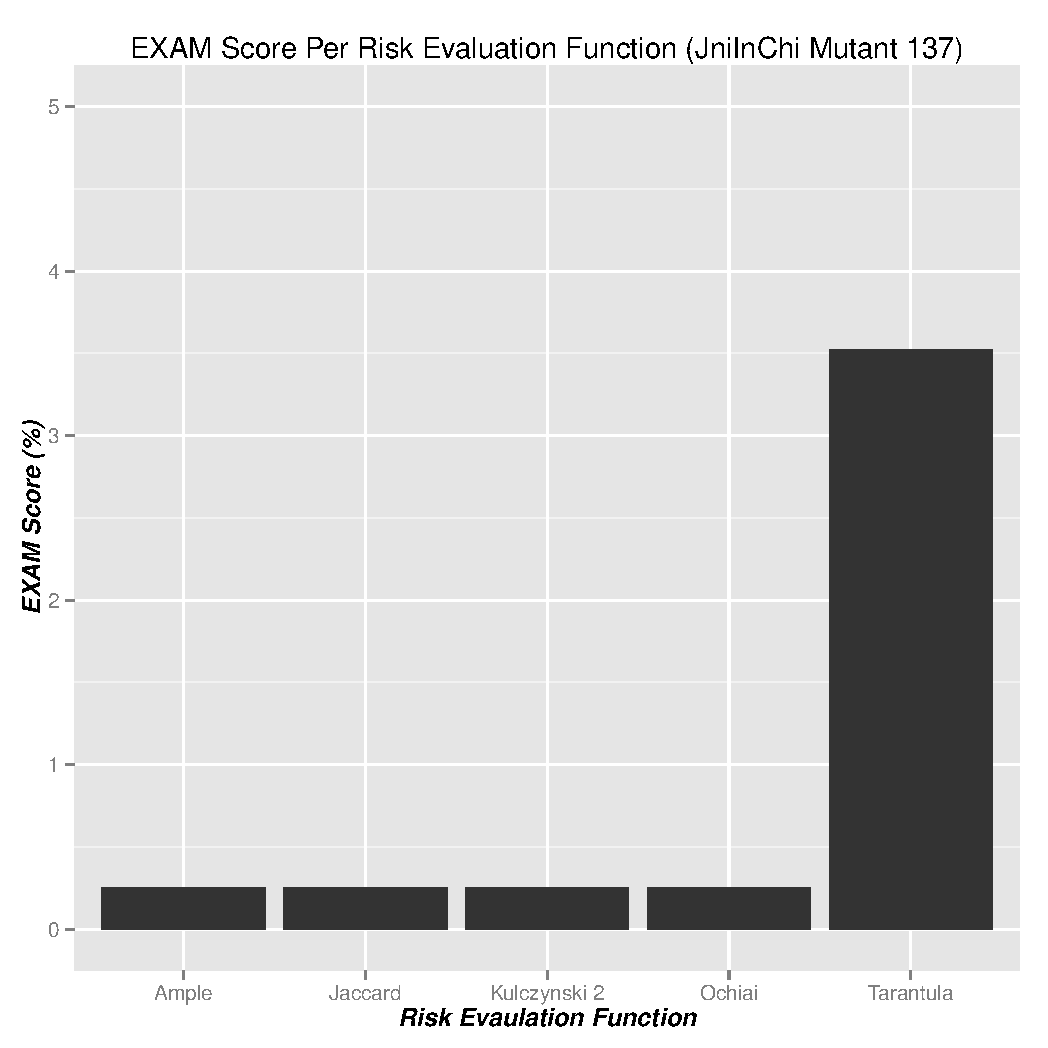
\includegraphics[width=0.4\linewidth]{img/graph_137.pdf}

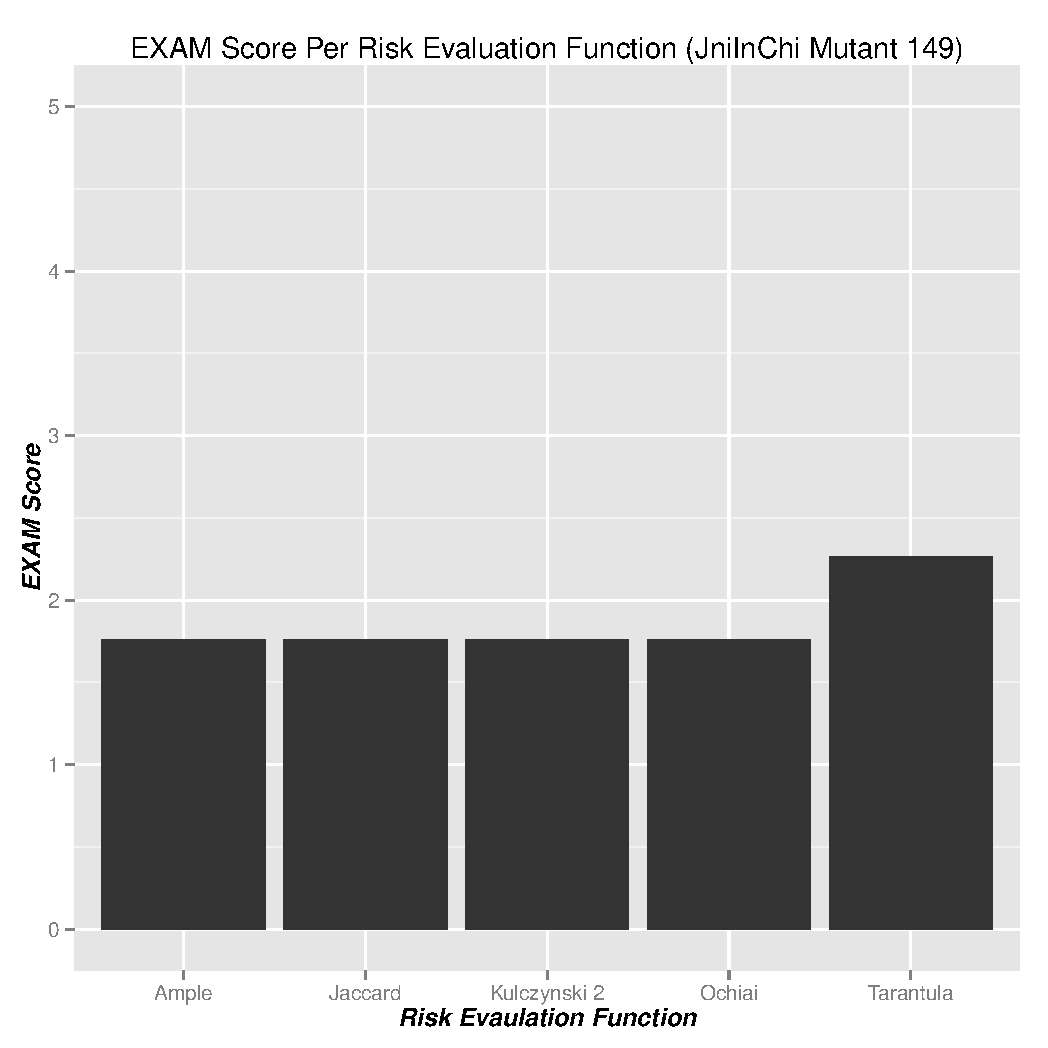
\includegraphics[width=0.4\linewidth]{img/graph_149.pdf}
\hspace{0.1\linewidth}
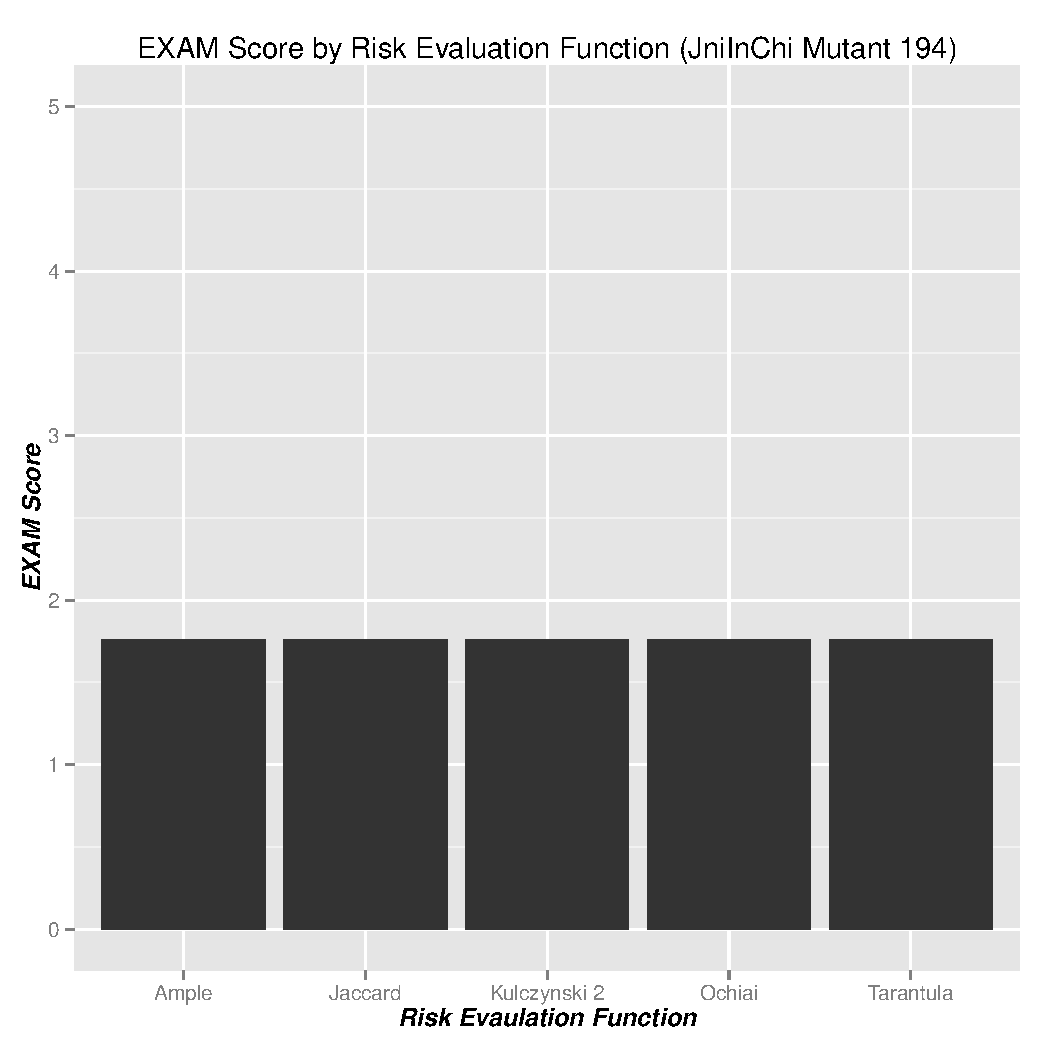
\includegraphics[width=0.4\linewidth]{img/graph_194.pdf}

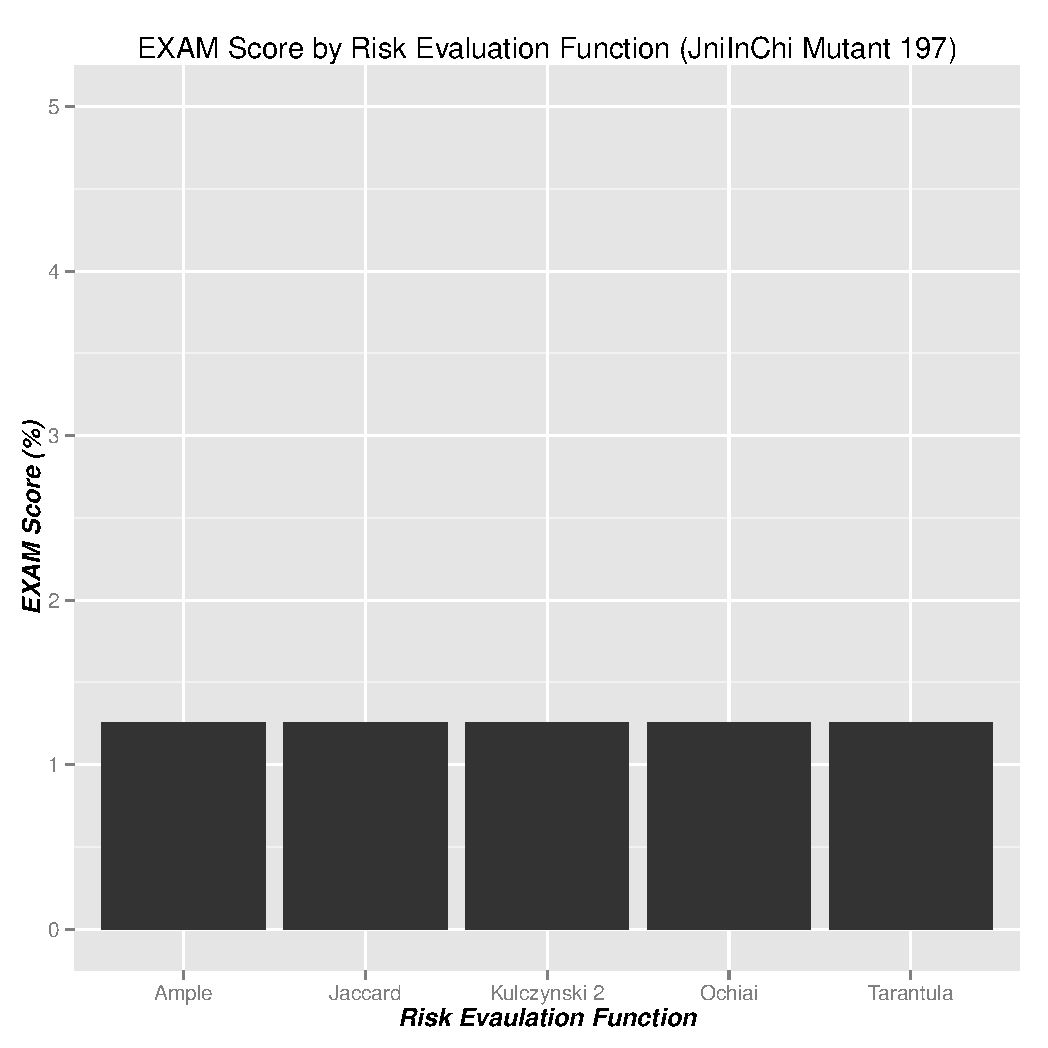
\includegraphics[width=0.4\linewidth]{img/graph_197.pdf}
\hspace{0.1\linewidth}
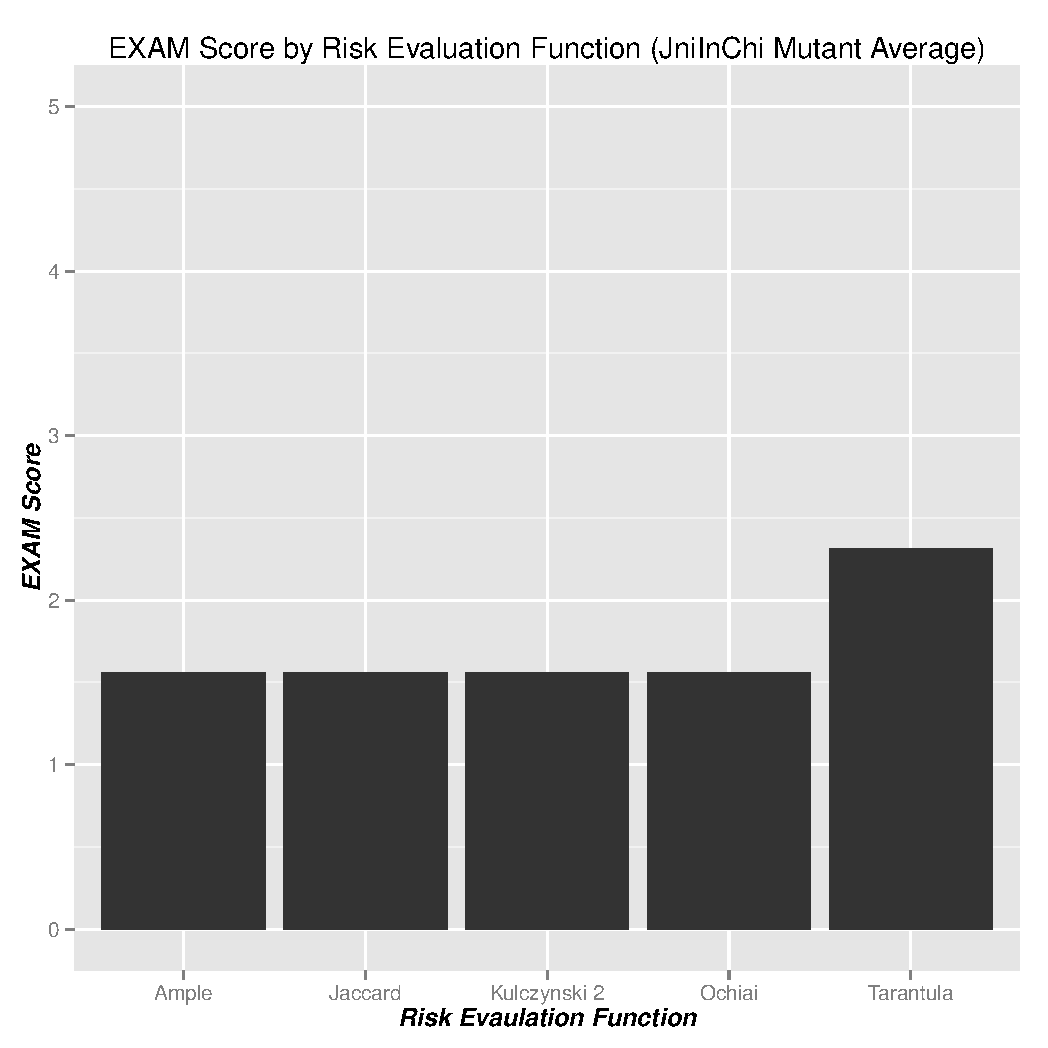
\includegraphics[width=0.4\linewidth]{img/graph_avg.pdf}

\caption{Graphs produced through R showing the results of running
the system on each selected mutation on our case study.  Each graph
shows the EXAM score achieved by each risk evaluation function for a
different mutant, with the exception of the last (lower right) which
shows average EXAM score overall for the case application.  All graphs
are fixed to the same EXAM range from 0\% to 5\%.}
\label{fig:results}
\end{figure}

The bar graph visualization of our results is can be found in Figure \ref{fig:results}.  For nearly every case, 
we notice that every risk evaluation function performed nearly or exactly the same.  Though the 
graph for Jni-InChi mutant 137 appears to be wildly skewed, it is important to note that the range of the
graph only covers five percent.  Even in the worst case, none of the risk evaluation functions scored
worse than 3.5\%.  Recall from Section \ref{sec:afl} that EXAM score is a lower-is-better metric
indicating the percent of statements that need to be visited, when proceeding sequentially through a 
list of suspicious statements, before encountering the actual faulty statement.


\section{Threats to Validity}\label{sec:valid}

Due to complications related to the use of CodeCover to generate per-test coverage, we were only able
to produce results for a single case application.  As such, we can only provide a certain degree of
confidence in the correctness and versatility of our system for processing CodeCover containers.  However,
after testing and developing the system with a very simple application, no modifications were necessary
to process the far more extensive output generated when running CodeCover on our case application.  This 
allows us to conclude that we can be reasonably confident that our system will likely work for any
coverage container.  The difficultly, then, lies in the limited capacity of CodeCover to produce 
output for a wide variety of source applications.

